\documentclass[border=3pt]{standalone}
% Preâmbulo compartilhado pelos diagramas TikZ da aula 14 (SLAM com EIF)
\usepackage[T1]{fontenc}
\usepackage[utf8]{inputenc}
\usepackage{lmodern}
\usepackage{amsmath}
\usepackage{xcolor}
\usepackage{tikz}
\usetikzlibrary{arrows.meta,angles,quotes,decorations.pathmorphing,decorations.pathreplacing,calc,
                positioning,shapes.geometric,shapes.misc,backgrounds,fit,
                math}

% Paleta (mesma dos SVGs originais)
\definecolor{dblue}{HTML}{2A5B8C}
\definecolor{dorange}{HTML}{B3541E}
\definecolor{dgreen}{HTML}{4A7C59}
\definecolor{dred}{HTML}{9C4B4B}
\definecolor{dcream}{HTML}{F4F1EA}
\definecolor{dshade}{HTML}{DDD7C9}

% Função gaussiana (não normalizada por padrão de escala visual)
\pgfmathdeclarefunction{gauss}{3}{%
  \pgfmathparse{1/(#3*sqrt(2*pi))*exp(-((#1-#2)^2)/(2*#3^2))}%
}

% Estilos comuns (prefixo d... para não colidir com chaves internas do pgf)
\tikzset{
  >={Stealth[length=2mm]},
  dguide/.style={gray!55, dashed, line width=0.4pt},
  daxis/.style={gray!60, line width=0.7pt, ->},
  dbody/.style={fill=black!3, draw=black!80, line width=1pt},
  dacc/.style={draw=dblue, line width=1pt},
  dlbl/.style={black!55, font=\small},
  dsub/.style={black!45, font=\footnotesize},
  dstate/.style={circle, draw=black!80, fill=dcream, line width=1pt,
                 minimum size=17mm, font=\large, inner sep=1pt},
  dobs/.style={circle, draw=black!80, fill=dshade, line width=1pt,
               minimum size=14mm, font=\large, inner sep=1pt},
  dbox/.style={rounded corners=2pt, draw=black!80, fill=dcream, line width=1pt,
               align=center, inner sep=6pt},
  dop/.style={circle, draw=black!80, fill=white, line width=1pt,
              minimum size=6mm, inner sep=0pt, font=\small},
  dtrans/.style={->, dblue, line width=1pt},
  dmeas/.style={->, dorange, line width=1pt},
  dcurve/.style={line width=1pt, dblue},
  dcurveb/.style={line width=1.4pt, dorange},
}

\begin{document}
\hyphenpenalty=10000 \exhyphenpenalty=10000 \tolerance=9999 \emergencystretch=3em
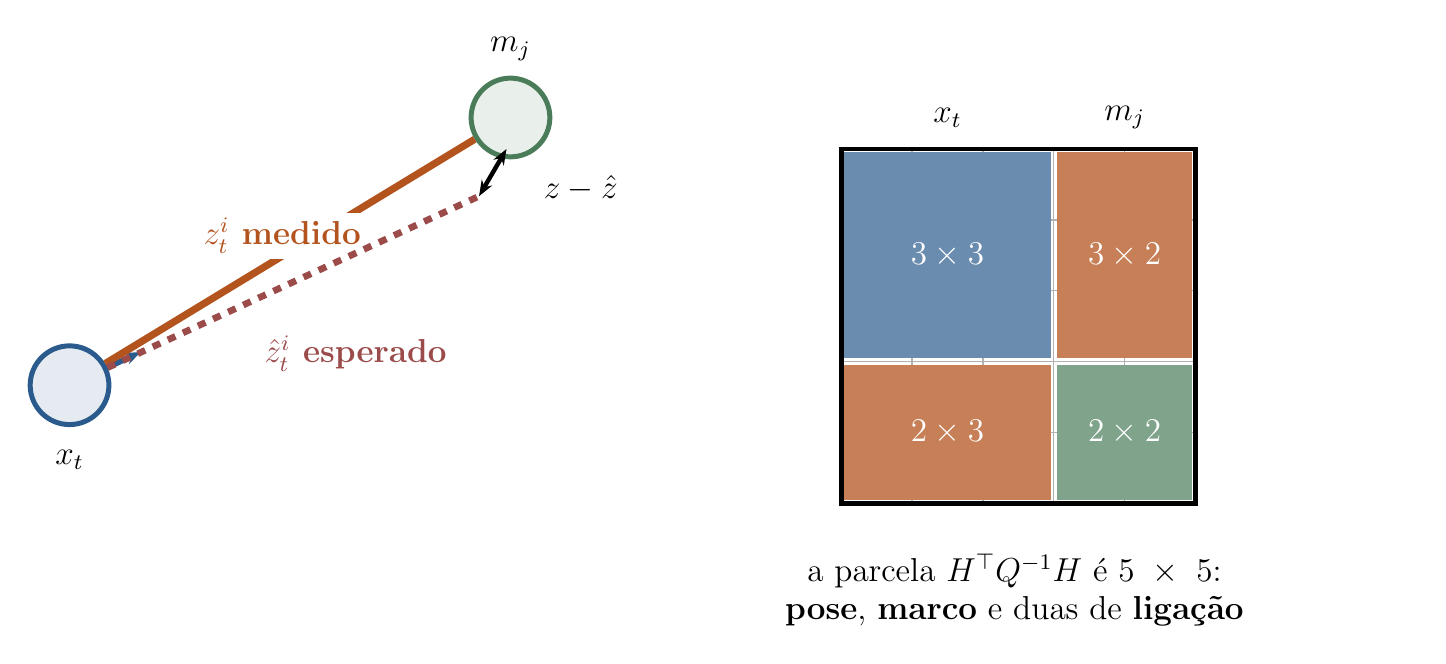
\begin{tikzpicture}[x=1cm,y=1cm]
\tikzset{p/.style={circle, draw=dblue, fill=dblue!12, line width=1.8pt, minimum size=1.0cm},
        m/.style={circle, draw=dgreen, fill=dgreen!12, line width=1.8pt, minimum size=1.0cm}}
\node[p] (r) at (1.8,2.0) {}; \draw[->, line width=2pt, draw=dblue] (r) -- ++(25:1.0);
\node[font=\large, anchor=north] at (1.8,1.3) {$x_t$};
\node[m] (l) at (7.4,5.4) {}; \node[font=\large, anchor=south] at (7.4,6.0) {$m_j$};
\draw[dorange, line width=2.6pt] (r) -- (l); \node[font=\large\bfseries, text=dorange, fill=white, inner sep=2pt] at (4.5,3.9) {$z_t^i$ medido};
\draw[dred, dashed, line width=2.4pt] (r) -- (7.0,4.4); \node[font=\large\bfseries, text=dred, fill=white, inner sep=2pt, anchor=west] at (4.2,2.4) {$\hat z_t^i$ esperado};
\draw[<->, line width=1.6pt] (7.0,4.4) -- (7.35,5.0); \node[font=\large, anchor=west] at (7.7,4.5) {$z-\hat z$};
\def\cw{0.9}
\foreach \i in {0,...,4} {\foreach \j in {0,...,4} {\draw[black!30, line width=0.5pt] ({11.6+\j*\cw},{5.0-\i*\cw}) rectangle ({11.6+(\j+1)*\cw},{5.0-(\i+1)*\cw});}}
\fill[dblue!70] (11.64,4.96) rectangle (14.26,2.34);
\fill[dgreen!70] (14.34,2.26) rectangle (16.06,0.54);
\fill[dorange!75] (14.34,4.96) rectangle (16.06,2.34); \fill[dorange!75] (11.64,2.26) rectangle (14.26,0.54);
\draw[line width=1.8pt] (11.6,5.0) rectangle (16.1,0.5);
\node[font=\large\bfseries, text=white] at (12.95,3.65) {$3\times3$};
\node[font=\large\bfseries, text=white] at (15.2,1.4) {$2\times2$};
\node[font=\large\bfseries, text=white] at (15.2,3.65) {$3\times2$}; \node[font=\large\bfseries, text=white] at (12.95,1.4) {$2\times3$};
\node[font=\large] at (12.95,5.4) {$x_t$}; \node[font=\large] at (15.2,5.4) {$m_j$};
\node[font=\large, text width=10cm, align=center] at (13.8,-0.6) {a parcela $H^\top Q^{-1}H$ é $5\times5$: \textbf{pose}, \textbf{marco} e duas de \textbf{ligação}};
\end{tikzpicture}
\end{document}
